\documentclass[twocolumn]{article}
\usepackage{graphicx} % Required for inserting images
\usepackage{hyperref}
\usepackage[utf8]{inputenc}
\usepackage{float}
\usepackage[margin={2cm,2cm}]{geometry}
\usepackage{xcolor} % to access the named colour LightGray
\definecolor{LightGray}{gray}{0.95}
\usepackage{minted}
\usepackage{caption}
\usepackage{cprotect}
\usepackage{csquotes}
\usepackage{listings}
\usepackage{color}
\lstset{
    showstringspaces=false,
    basicstyle=\ttfamily,
    keywordstyle=\color{blue},
    commentstyle=\color[grey]{0.6},
    stringstyle=\color[RGB]{255,150,75}
}
\usepackage[
sorting=none
]{biblatex}
\addbibresource{references.bib}
\usepackage[toc,page]{appendix}


% Automated the Figure referencing and make it fully clickable
% \newcommand{\FigRef}[1]{Figure~\ref{#1}}
\newcommand{\FigRef}[1]{\hyperref[#1]{Figure~\ref{#1}}}

\newcommand{\inlinecode}[2]{\colorbox{LightGray}{\lstinline[language=#1]$#2$}}

\newenvironment{code}{\captionsetup{type=figure}}{}

\renewenvironment{abstract}
 {\par\noindent{\Large\textbf{\abstractname}}\par \vspace{1em}}
 {\par\noindent\medskip}

\makeatletter
\renewcommand{\maketitle}{
  % Center the title (default behavior)
  \begin{center}
    \LARGE \textbf{\@title}
  \end{center}
  % Left-align the author and date
  \vspace{0.4cm}
  \begin{flushleft}
    \@author \\[0.5em]  % Optional: adds space after author
    \@date
  \end{flushleft}
}
\makeatother

\title{
    Virtual machine to container migration system
}
\author{
    Antonio Takev \\
    \href{mailto:a.takev@student.fontys.nl}{a.takev@student.fontys.nl} \\
    Master of Applied IT, Fontys University
}
\date{January 2025, Eindhoven, Netherlands}

\begin{document}

\twocolumn[
\begin{@twocolumnfalse}
    \maketitle

    {\color{gray}\hrule}
    \vspace{0.4cm}
    \begin{abstract}
    In software engineering, containers have become very popular in the last few years due to their advantages such as increased portability, operational stability, and lightweight design, over virtual machines. Although companies started migrating their application from virtual machines to containers and consequently, Kubernetes clusters, it was discovered there is a shortage of tools and knowledge on automating such migrations. The goal of the paper is to design the software architecture and infrastructure of a system that can perform automated black-box migrations of applications from virtual machines to containers. The paper describes the successful construction of an enterprise-level software system that can transfer a stateless application such as a web server from an Ubuntu-based virtual machine to a Docker container, achieved by combining system analysis and design, expert evaluation, prototyping, and testing as a cycle-based methodology to tackle the issue. More research needs to be completed to enhance the business logic of the system so that it can migrate more complex stateless and stateful applications. Different aspects of the system's life cycle such as Black-box migration, Software architecture, Software design patterns, User experience, and Infrastructure management were examined to form a solution that is flexible, extensible, user-friendly, and can be the basis of an innovative way to modernize through containerization software applications owned or managed by companies of all sizes.
    \end{abstract}

    \vspace{1em} % Space after abstract
    \noindent\textbf{Keywords:} \textbf{virtual machine, containerization, black-box migration, analysis, file system analysis, dockerization, software architecture} \\
    {\color{gray}\hrule}
    \vspace{0.4cm}
\end{@twocolumnfalse}
]

\section{Introduction}
The software industry is continuously growing and has gone through a natural evolution from native to virtualized, to cloud, and now to container technology, making the term containerization quite popular among developers and companies of all sizes \cite{SiddiquiEtAl-2020}. Containerization is a method for virtualizing programs \cite{VermaEtAl-2022} and the container, defined by \cite{GargEtAl-2024}, is a lightweight alternative to virtual machines to co-host multiple applications on a single server. The shipment of containers-based applications makes them available, tested and deployed on many servers \cite{VermaEtAl-2022} providing independent plans for upgrades and maintenance \cite{SiddiquiEtAl-2020}. Before containers, developers had to face many challenges when migrating an application from one virtual machine (VM) environment to another as usually, no two environments are similar in terms of both software and hardware capabilities \cite{SiddiquiEtAl-2020} and it is hard to examine what is running and had been installed on the virtual machine so that it can be replicated in the new environment. \\

As containerization gained popularity, many companies started migrating from virtual machines to containers for their legacy applications. The topic is not new, and there are some technologies like KubeVirt, Virtlet, and RancherVM which at first glance seem to work on the issue of automated migrations. However, they do not make any migration, instead, they provide a way to run virtual machines in Kubernetes clusters directly (KubeVirt, Virtlet)\cite{Sheldon-2022} or by packaging them in Docker images (RancherVM) \cite{Baccini-2021}. The only product that provides a tool to make an actual migration is Migrate to Containers \cite{Google-2024}, offered by Google Cloud. However, this tool works in the close-sourced environment of Google, and it can be used only if the migration of an application from VM to container will be performed within the Google Cloud ecosystem. \\

Considering the lack of tools or systems to migrate applications, residing in virtual machines, to containers, the research paper takes this as the main research gap. While automation issues are usually considered problems that can be solved through scripts, this research paper aims to go beyond this and investigate the possibilities of designing an enterprise-level system that can transfer applications from virtual machines to containers, focusing on different topics that have to complete the system's life cycle. Moreover, the system will introduce the term "black-box migration", used to describe that the system can perform a migration without or with minimum prior knowledge of the type, structure, and technical stack of the application to be migrated. \\

In the paper, several segments of the system will be closely examined as separate but connected topics: Black-box migration, Software architecture design, Software design patterns, User experience, and Infrastructure management. The research paper aims to design the software architecture and infrastructure of a software system that automates the process of migrating stateless applications from virtual machines to containers so that the applications can be deployed in Kubernetes clusters.

\subsection{Industry case}
Concerning the goal of this paper of automating the migration of applications from virtual machines to containers, a closer examination of the industry aspect of the problem was made. Many companies moved some or all of their applications from virtual machines to containers and eventually, Kubernetes clusters, and one good example is Sue. \\

Sue is a Netherlands-based company that specializes in cloud-native technologies. They have built a cloud platform called Multistax, which hosts applications on Kubernetes clusters to use the power of containers. However, around 70\% of their workloads at the moment are still residing on virtual machines, and they need a way to migrate all their applications, located on virtual machines, to containers. To modernize its infrastructure and apply containerization, companies like Sue aim to automate the process of migrating applications from virtual machines to containers, and therefore Kubernetes clusters. \\

To cover all this, Sue has created the project 'Application Profile' to investigate how to gather the various dependencies, components, and configurations necessary for a migration of an application from a virtual machine to a containerized environment. During the first iteration of the project, a group of students from the Bachelor’s in ICT\footnote{ICT - Information and communications technologies covers all technical means used to handle information and aid communication} and Software Engineering at Fontys University of Applied Sciences developed a tool that could extract and describe the files and packages from a VM and generate a Dockerfile. The tool was built to gather a list of packages, configuration, and application files from a VM and then build a Dockerfile based on them using AI, and more specifically ChatGPT. The solution required manual work and it was not extensible, which made the stakeholders from Sue not so confident in the advantages of using AI to fulfill the project needs. \\

As a sponsor for this research, the goal of the stakeholders from Sue is to overcome the limitations of the first iteration by automating the generation of an application profile and the creation of a container based on it.

\section{Literature review}
To provide an automated solution to transfer applications from virtual machines to containers, the study began by defining some terminology behind the migration process and the concepts of containers and virtual machines. \\

The concept of containerization, as stated in \cite{Bhat-2022}, can be found in early 1979 with the introduction of UNIX\footnote{UNIX - It is a family of multitasking, multi-user computer operating systems} Version 7 which allowed process isolation by changing the root directory of a process. As stated in \cite{SiddiquiEtAl-2020}, the use of containers results in operational efficiency as containers package the applications with all their required dependencies in terms of software, libraries, configuration files, binaries, and other required data to execute the application. This helps developers run the application in any environment already shipped with all its dependencies \cite{SiddiquiEtAl-2020}, and the use of a container benefits both the development and deployment of software \cite{VermaEtAl-2022}. \\ 

In the context of containers, there are two main terms: an image and a container. Defined by \cite{HaleEtAl-2017}, an image is an immutable file that contains a description of a complete computing environment (e.g., libraries, executables, default networking configuration) that can be used by a runtime such as Docker to create a container. A container, as specified in \cite{HaleEtAl-2017}, is a runtime instantiation of a particular image and it is possible to have many containers based on the same image. As described in \cite{HaleEtAl-2017}, an image can be built using a Dockerfile, a sequence of some Docker-specific directives and shell script commands that prescribe the entire build process and runtime configuration of a software environment. \\

The transition from VM-based to container-based environments is gaining traction, as containers provide better performance and resource efficiency while still addressing challenges like isolation and dependability \cite{GargEtAl-2024}. As mentioned in \cite{Yade-2022}, containers are more portable as they run in every environment, and faster as they run almost instantly. Containers being a packaging unit for any application and producing operating system level virtualization \cite{SiddiquiEtAl-2020}, can be viewed as a core principle of achieving system deployments and runtime portability across different operating systems which is another reason for the active integration of the container technology. \\

There are several well-known tools to make use of virtual machines in Kubernetes clusters, examples of which are KubeVirt, Virtlet \cite{Sheldon-2022}, and RancherVM \cite{Baccini-2021}, but they do not perform any migration. They place already functioning virtual machines into more complicated environments like Kubernetes clusters, eventually producing bugs and increasing complexity. \\

The research found only one tool (Migrate to Containers\cite{Google-2024}) that can perform a migration of an application, which resides in a virtual machine, to a container. Written in \cite{Google-2024}, Google Migrate to Containers is a tool designed to convert VM-based workloads into containers within Google Kubernetes Engine (GKE) or GKE Enterprise. This tool supports migrating workloads from on-premises VMware environments or Google Computer Engine \cite{Google-2024}, while tools like RancherVM provide a solution for packaging and running VMs as Docker containers \cite{Baccini-2021}, thus allowing VMs to be managed as if they were containers within Docker. KubeVirt allows the management of applications residing in VMs through Kubernetes by enabling VMs to be run as Kubernetes pods \cite{Sheldon-2022}. Virtlet is a similar tool \cite{Sheldon-2022} that is not anymore maintained according to their official \href{Github repository}{https://github.com/Mirantis/virtlet}. \\

Google Migrate to Containers supports the modernization of the following workloads: Linux VM containers, Linux-based workloads (Tomcat, Apache, JBoss, WebSphere, WordPress sites), and Windows IIS applications \cite{Google-2024}. Migrate to Containers by Google supports migrations of VMs to containers on Google Kubernetes Engine on the following 64-bit Linux operating systems: CentOS, Debian, RHEL, SUSE, and Ubuntu \cite{Google-2024}. The tool supports all Linux-based operating systems for Linux-based workloads \cite{Google-2024}. Google Migrate to Containers provides possibilities to migrate VMs to containers on different Linux distributions through a CLI\footnote{CLI - Command line interface, a mechanism to interact with a computer program by using lines of text, called command lines, as an input} tool that collects the file system of the target VM where the application to be transferred is located \cite{Google-2024}. \\

In the documentation of Google Migrate to Containers \cite{Google-2024}, it is stated that they copy the file system of the target machine and perform analysis on it. In the paper this approach will be recalled under the name: "file system analysis" and it can be used in the solution to migrate an application from a VM to a container. In Linux, everything is a file \cite{Torvalds-2002}, which indicates a migration approach based on file system analysis can get the application files, exposed ports, and services, used by an application that has to be transferred from a virtual machine environment to a container environment. \\

In all operating systems, there is one abstraction, called process, which can be defined as an "instance of a program in execution" or as "the execution context" of a running program \cite{BovetEtAl-2005} which provides a second option to see what an application is using in terms of application files, exposed ports, and services. The second approach of collecting application data by performing analysis on the target VM will be referred to in the paper as "process analysis".

\subsection{Software architecture and software design patterns}
The analysis part is the core of the migration process but to design a migration system, the first step is to organize its components into a software architecture. Software architecture plays a main role in providing scalability and maintainability and aligning technical decisions with business objectives \cite{Nivedhaa-2024}. \\

Recent trends emphasize microservices, and cloud-native architectures as key approaches to achieve these goals \cite{Nivedhaa-2024} and modular monolith as an approach which is gaining popularity \cite{SuEtAl-2024}. Summarized by \cite{Nivedhaa-2024}, modularity, loose coupling, and high cohesion are some of the best practices to make a scalable and fault-tolerant software system. In the world of enterprise-level software systems, big and small companies tried microservices. \cite{SuEtAl-2024} shared that some gained advantages like independent development and deployment of the core units of their software, while others did not get the expected benefits and experienced issues such as high costs and complexity of the system. In \cite{SuEtAl-2024} it was explained that modular monoliths are organized in well-defined, isolated modules that can be worked independently but deployed as a single unit. \\

The well-known principle of separation of concerns (SoC) can be used to decompose software systems into manageable units \cite{Daga-2006}, particularly useful in the context of an enterprise-level migration system that has the potential to grow and improve its success rate. Decomposition of the system into units will help achieve ease of change, more localized maintenance, and reuse \cite{Daga-2006}. Going more in-depth into the solution, people usually try to solve commonly occurring problems in their systems. Such issues can be solved through the use of design patterns. By definition, design patterns are well-known and good solutions to a common problem \cite{Martin-2000} and provide several benefits such as reusable software, reduced complexity, reduction of learning time, and helping novices perform like experts \cite{GammaEtAl-1993}. \\

Design patterns gained popularity through OOP\footnote{OOP - Object-oriented programming is a computer programming paradigm that organizes software design around data, or objects, rather than functions and logic} and the trend of using various principles and best practices to make the code base more powerful and future-proven. Design patterns vary in their purpose and goals and are commonly organized in the following families: Creational, Structural, and Behavioral \cite{GammaEtAl-1993}. They can be used alone or in combination no matter which family they originate from. The Creational family abstracts how objects are used by hiding the specifics of the creation process, the Behavioral design patterns focus on the relationship between objects or classes, and the Structural patterns are used to combine objects and classes into larger structures while keeping them flexible \cite{GammaEtAl-1993}. 

\section{Methodology}
To design a software system to migrate an application from a virtual machine to a container a custom Agile-inspired approach with four phases was modeled \FigRef{fig:work_approach} combining different research methods, the Technology Impact Cycle Tool (TICT) for Ethical check, and the Agile mindset.

\begin{figure}[H]
    \centering
    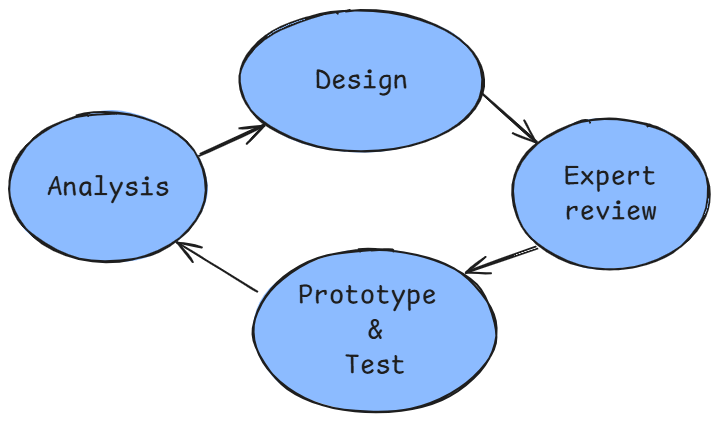
\includegraphics[width=\linewidth]{images/approach.png}
    \caption{Work Approach}
    \label{fig:work_approach}
\end{figure}

By design, Agile is a way to respond to changes and succeed in an uncertain and turbulent environment, and as the Agile Manifesto stands \cite{BeckEtAl-2001}, the aim is to deliver results by frequently promoting reflection on work at regular intervals of time and maintaining a constant working pace. Similarly to how software development works, in the academic research domain, the project context, direction, and requirements continuously change based on the findings and experiments, which requires a flexible research approach with the possibility to go back and forth and make adjustments. \\

The research approach consists of the following phases: Analysis, Design, Expert review, and Prototype \& Test. The approach is in the form of a cycle of these steps which is completed once the results are satisfying. During the Analysis phase, the problem and context of this research paper were closely examined and a thorough background research was performed on the topics of containerization, application profiling, and software architecture. To find the well-known architecture styles, best practices in the architecture design, or ideas, rules, and trends for making user-friendly command-line interfaces, a literature review was performed. In addition to the literature review, design pattern research was also utilized to design the system to be extensible and flexible, and the code base to be organized and following best practices in the enterprise software domain. Detailed background research on the topics of containerization, migration strategies, architecture design, and design patterns was conducted. During the analysis phase, an Ethical check was also performed. \\

The system's architecture design was set as a primary goal from the start which required the IT architecture of the system to be sketched so that the system can perform a black-box migration of an application from VM to container. During the design phase, various well-known architectural styles such as Monolithic, N-layer, Headless, and Microservices were examined and mixed to provide several suggestions for a custom-based architectural style that fulfills the system requirements. \\

To make the system more flexible and extensible, two software design patterns were integrated. To design the system for the user needs, a close look at the user experience was taken, searching for best practices in organizing the software components of the system so that it remains lightweight and loosely coupled. The designs were discussed with experts from the industry field and professors in the area of software engineering and infrastructure from Fontys University. \\

As a natural consequence of the design step, prototyping was used to build a proof of concept (PoC) to showcase the system component of black-box migration using file system analysis as a main migration approach. To prove the software design of the system the PoC was developed to be able to migrate a Nginx web server as a traditional example of a stateless application. The web server was deployed on a Virtual machine with Ubuntu 22.04 (a well-known Linux flavor) on Google Cloud and SSH access was provided. The goal of the PoC was to analyze the VM and find the application files, ports, and services of the web server and then create an application profile which results in a fully-working Docker container that packages the web server. The PoC was tested to see how complete the result of migrating a Nginx web server from a Ubuntu VM to a Docker container was. \\

The last point of the research methodology was to design and explain the infrastructure strategy for managing the system components. \\

Considering the complex objective of this paper to design the complete life cycle of a system to perform migrations, the results were presented into several sections: Black-box migration, Software architecture, Software Design patterns, User experience, and Infrastructure management, starting with a brief introduction to what the study accomplished. All these sections highlight different areas of the system's life cycle and help the reader dive deeper into it.

\subsection{Ethical check}
An ethical check on the system was performed to introduce some insights into whether the system was built to support user's needs while keeping its functionalities legitimate. In terms of human values, it was determined the system can replace the manual process of migrating an application from a VM to a container in a more automated way. As a result, users of the system (usually software developers and DevOps/Cloud specialists) can be empowered to produce modern deployment strategies for clients whose legacy applications are still residing in VMs. Moreover, companies using the system can focus on clients' real desires and "pains".\\

The main stakeholders for the system appeared to be companies that would like to migrate their applications from virtual machines to containers in an automated way. As a sponsor of the project, Sue and the employees working there were considered as main stakeholders for the project, represented by the Product owner of the project - Nathan Keyaerts. They continuously provided both academic and technical feedback but also business-oriented advice which in terms of ethical view can change the direction of a project.\\

If the system was designed for the employees working at a specific company, this immediately could have formed a bias based on their demographics and financial status. A more generic approach was needed to exclude such bias and to provide a system that can be used by more than one company. Different companies might like to take a different approach when solving the issue but making the system to be extensible in terms of migration approaches was a point in the right direction.\\

Regarding data management, the system was not designed to use any sort of data collection, because it provides a way to automate the process of migrating an application from a VM to a container which indicates that every application is unique and contains real data in this sense. As personal data, GDPR, and privacy are important topics for a system that aims to migrate real applications, a closer look at who uses the system needs to be taken if the system is determined to be used in real-life scenarios. The technology can register personal data if the application contains a self-contained database or other type of data sources. Most probably this data would be already encrypted. To avoid any GDPR-related issues, the system must be used only by the employees at the company integrating the PoC of this research paper into their infrastructure.\\ 

If this system is determined useful, then it might be acquired by other companies that have similar issues as Sue. Additionally, it can be designed to serve a bigger amount of users and ideally save a lot of time for big and small companies, allowing the employees to focus on tasks requiring more in-depth work.

\section{Results}
 As a result of various software design and implementation cycles of applied experiments, an enterprise-level software system was designed using system diagrams and developed in the form of a PoC to allow users to migrate stateless applications from virtual machines to containers using the system's user-friendly interface.

\subsection{Black-box migration}
The brain of the system, its business/service logic, was assembled with the concept of making the system apply black-box migrations in a highly automated manner and producing a working container in the end. Using minimal user input, asking only for the username, IP, and SSH key to access the VM, the system was designed to perform black-box migrations. It was discovered that two main parts are required to perform automated migrations: analysis of what application needs to work in terms of files and other configurations, and containerization of the analysis output. To simplify the names of these parts, they were introduced in the system as \textbf{Analyze} and \textbf{Dockerize} sections. \\

The "Analyze" section is responsible for analyzing the VM and performing application profiling of the application. It analyzes what the application requires to be executed successfully outside of the VM and generates a profile out of it in the form of an output directory. The "Dockerize" section assembles a Docker container that packages the application and all its dependencies based on the application profile generated by the "Analyze" section. \\

The experiments applied within this research discovered that the "Analyze" process can bring a good percentage of success rate if it considers the following segments to profile: application files, exposed ports, and system services. Application files are needed to run the application successfully outside of the VM. The ports the application uses need to be exposed in the container to make the application available. System services need to be started in the container as usually, the application is dependent on one or more system services to provide the desired functionality. \\

The business logic of the system was implemented in the form of a PoC which performs a black migration for a stateless application from the perspective of an enterprise-level software system. The PoC was built to be extensible and support more than one migration approach - file system analysis and process analysis. To make the system flexible, the approaches were designed to be interchangeable. In contrast, the option for a mixed approach was added to allow users to choose if they want certain parts of the analysis process to be taken by the \textbf{file system analysis} approach and others by the \textbf{process analysis approach}. \\

In the prototype, the file system analysis approach was only researched, designed, and developed in detail to minimize the scope and dive more into the business logic of the migration. As a matter of choice, the file system analysis was chosen as the analysis approach to be worked on in the paper as the other approach (process analysis) was researched on its own by another researcher, part of the same research group working on the project. The prototype successfully performed the migration of a Nginx web server, located in an Ubuntu VM, to a Docker container which was run and tested. \\

Shown in \FigRef{fig:data-colleciton}, the PoC, more specifically the \textbf{Analyze} package used different tools to support the successful collection of all the needed data for migration. 

\begin{figure}[H]
    \centering
    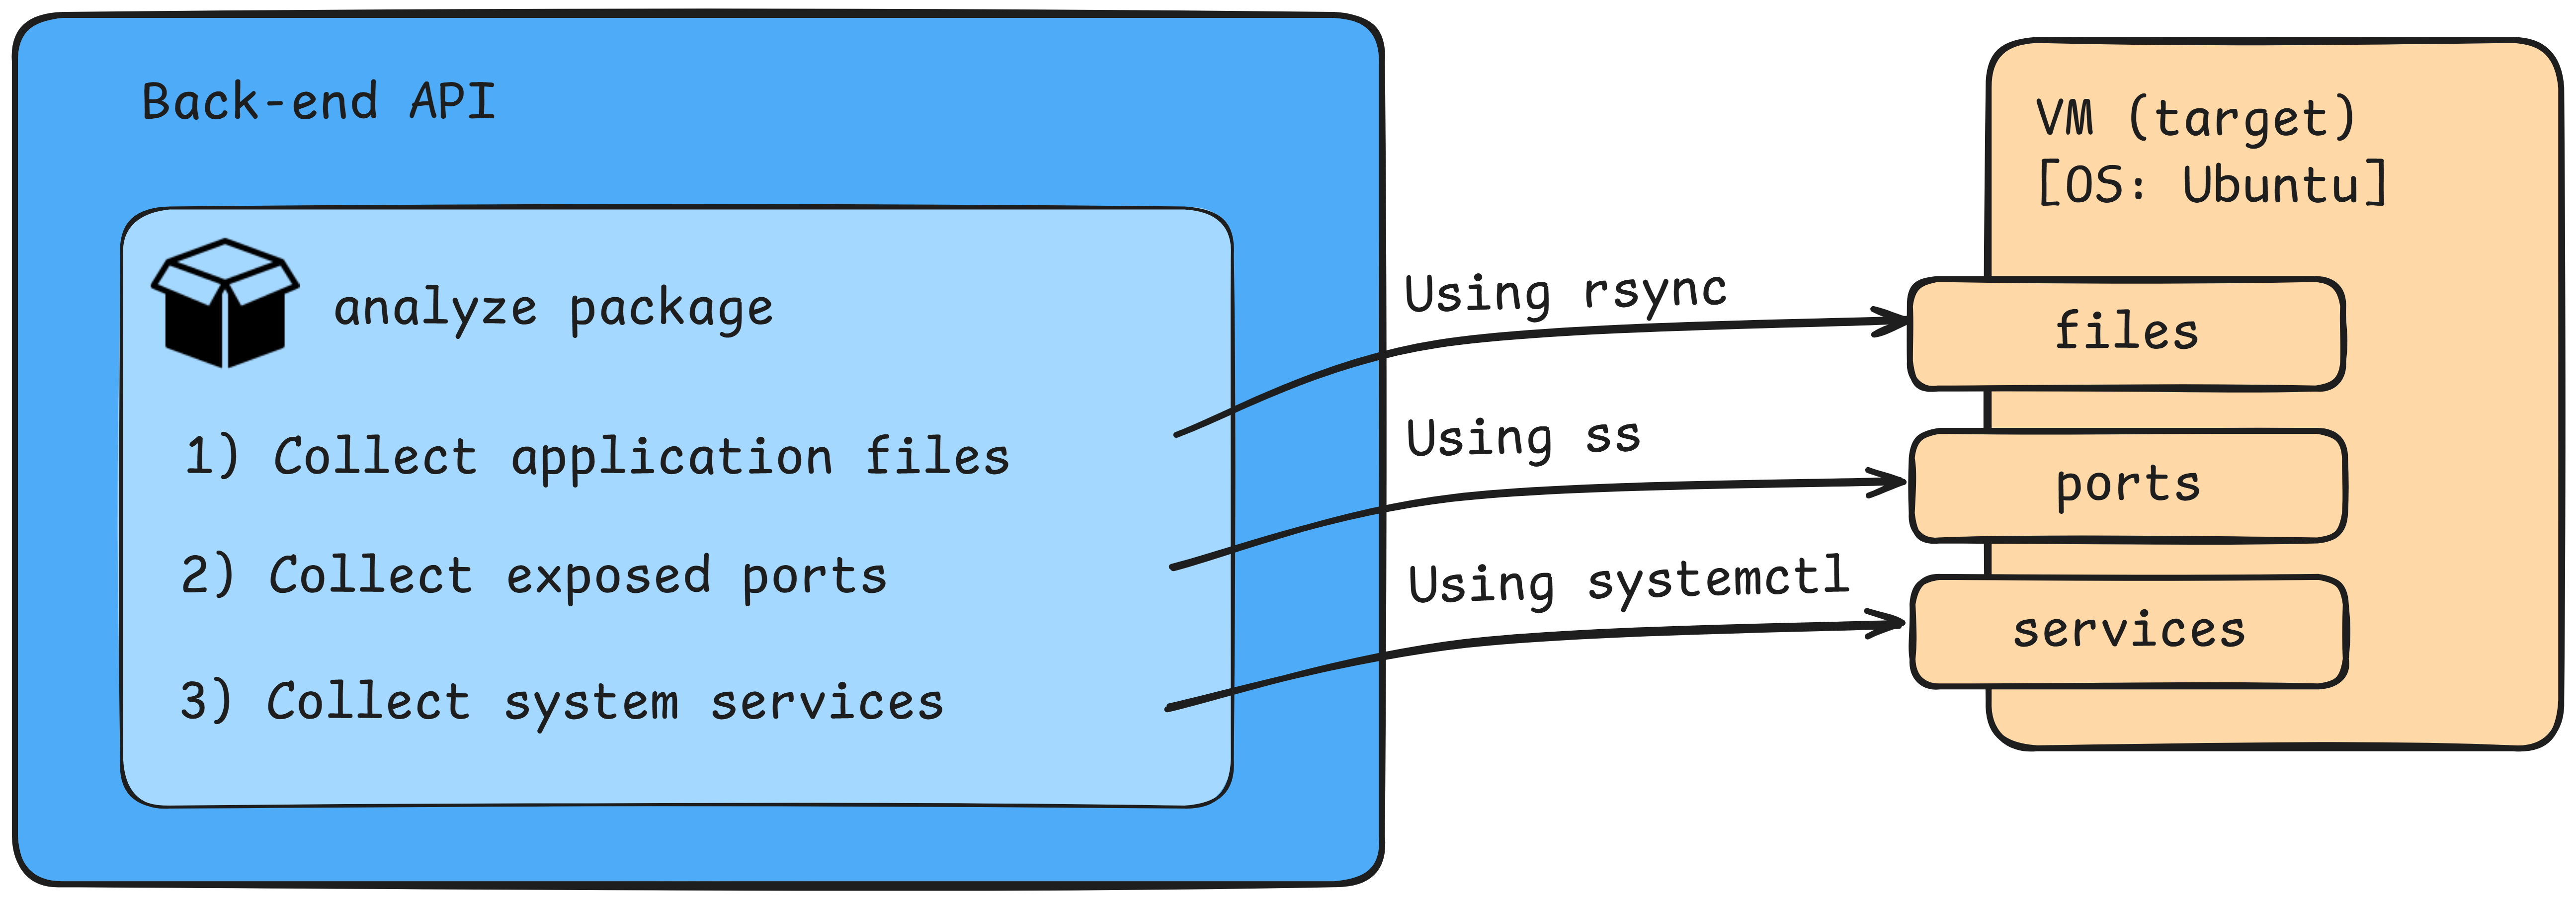
\includegraphics[width=\linewidth]{images/data-collection.png}
    \caption{Collection of data (app. files, ports, services)}
    \label{fig:data-colleciton}
\end{figure}

The collection of application files was made using the copying tool "rsync" which copies files and directories from the target VM to an output directory through SSH. The exposed ports were collected using the "ss" Linux command, which stands for Socket Statistics. Socket Statistics is a tool for inspecting and displaying detailed information about network sockets in Linux environments. To collect the running services on the target VM, the "systemctl" command was utilized together with some other tools to prepare the list of services for processing from the \textbf{Dockerize} package.

\subsection{Software architecture}
The system was designed with two components: a command-line interface (CLI) with which the user can interact, and a core unit that handles the business logic of the system. During the architecture design phase, several architectural styles were examined and their advantages and disadvantages were outlined so that in the end one architectural style or a mix can be selected and developed as part of the technical experiment of the research paper.

\subsubsection{Monolithic and N-layer monolithic architecture}
The two main components of the system: CLI and back end could be placed in one monolithic system \FigRef{fig:monolithic-architecture} which hints both of them will be developed and deployed together.

\begin{figure}[H]
    \centering
    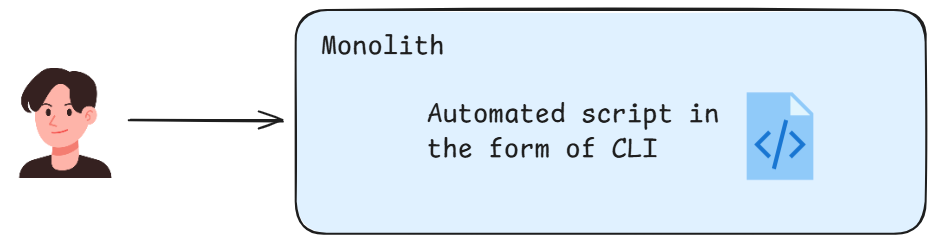
\includegraphics[width=\linewidth]{images/monolithic-architecture.png}
    \caption{Monolithic architecture}
    \label{fig:monolithic-architecture}
\end{figure}

By employing this approach the developer can write the service logic directly in the CLI. The approach can be extended by using SOLID principles and SoC and detaching the service logic from the CLI by organizing the code base into layers, inspired by the N-layer architecture style \FigRef{fig:n-layer-monolithic-architecture}. The system can be packaged as an all-in-one CLI tool which can be either installed as an executable/binary or accessed through a web interface by the user.

\begin{figure}[H]
    \centering
    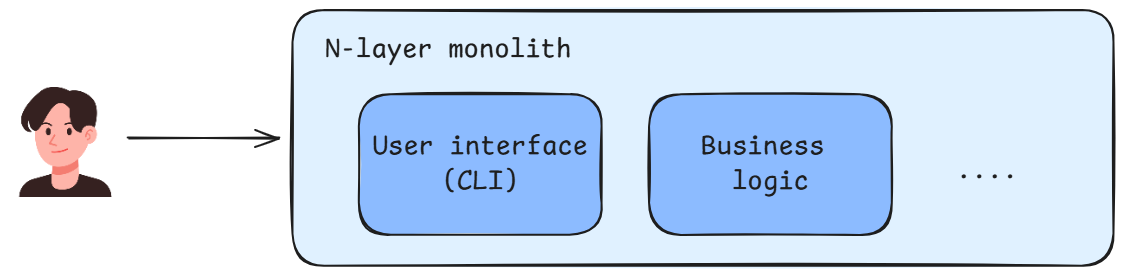
\includegraphics[width=\linewidth]{images/n-layer-architecture.png}
    \caption{N-layer Monolithic architecture}
    \label{fig:n-layer-monolithic-architecture}
\end{figure}

In the case of utilizing a monolithic architecture style, the main issue is the future view as the system components - CLI and back end cannot be developed or deployed independently. Moreover, it is difficult to update and maintain them, hard to extend them and there is the risk of making the CLI too heavy so that the users will lose satisfaction and will stop downloading and using it. The code for all the system components, which handles both analyze and dockerize parts of the migration process, could be placed in the same code base. This is a convenient benefit because it makes building a PoC a quick and easy challenge. \\

Additionally, the pure monolithic design of the system allows for organizing the back end in the form of an automated script that can print logs and messages to the console and improve user interaction. However, constructing the system as non-extensible and non-flexible because of the disadvantages in the monolithic design, makes this architecture style not suitable for the goals of the paper.

\subsubsection{Headless architecture}
In contrast to the Monoliths, Headless architecture \FigRef{fig:headless-architecture} is a modern style to separate the front end and the back end of an application \cite{Pachiyappan-2020}.

\begin{figure}[H]
    \centering
    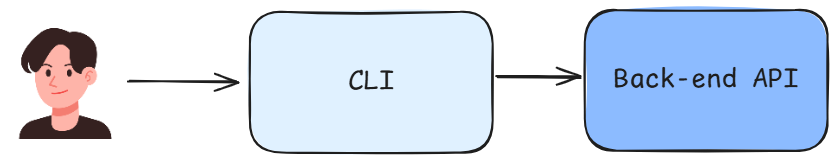
\includegraphics[width=\linewidth]{images/headless-architecture.png}
    \caption{Headless architecture}
    \label{fig:headless-architecture}
\end{figure}

The same principle can be employed to design the migration system as the CLI can act as the front end and the core unit can be the back end of the system. In this case, the two layers will be only able to communicate through an API. This adds more flexibility as the developer has the freedom to choose different technological stacks for each layer, and each layer can scale independently. \\

By separating the layers, the CLI can become much more lightweight, and user-friendly as it will only provide an interface for the user to interact with the system, while the back end can be deployed on a server on the company's infrastructure or in a cloud environment. This will also improve the performance of the CLI and result in people having to install a CLI tool that is very tiny which increases the likelihood of people using the system more often.

\subsubsection{Headless Microservice architecture}
In today's world microservice architecture style is recognized as an approach that organizes an application as a collection of two or more services that are independently deployable, loosely coupled, and organized around business capabilities \cite{Thönes-2015}. This would indicate separating firstly the front end (CLI) and the back end and then the back end will be further separated into two or more services. For example, the back end can be organized into "Analyze" and "Dockerize" services, each responsible for different parts of the migration. In the future, more services could be integrated such as Test service (responsible for testing if the migration was successful through various automated testing techniques) or Portability service (responsible for investigating the type of operating system (OS) the application is residing in and adding support for not only Linux Ubuntu but also other flavors and even other operating systems like macOS or Windows). This requires each service to be highly detached from the system and it is only reasonable if the system has a lot of service logic (also referred to in the paper as business logic) or multiple different components. \\

However, this is not the case for the current state of the system designed to serve more as a PoC. Another reason for not choosing this style is that it requires more costs to deploy every service and manage it. It will also add complexity in terms of communication between the modules as the middle layer needs to be introduced to synchronize their work and apply messaging. \\

In the context of the project, a combination of Headless and Microservice architecture styles could be a future suggestion in case the system expands in terms of functionality and business logic complexity \FigRef{fig:headless-microservice-architecture}. 

\begin{figure}[H]
    \centering
    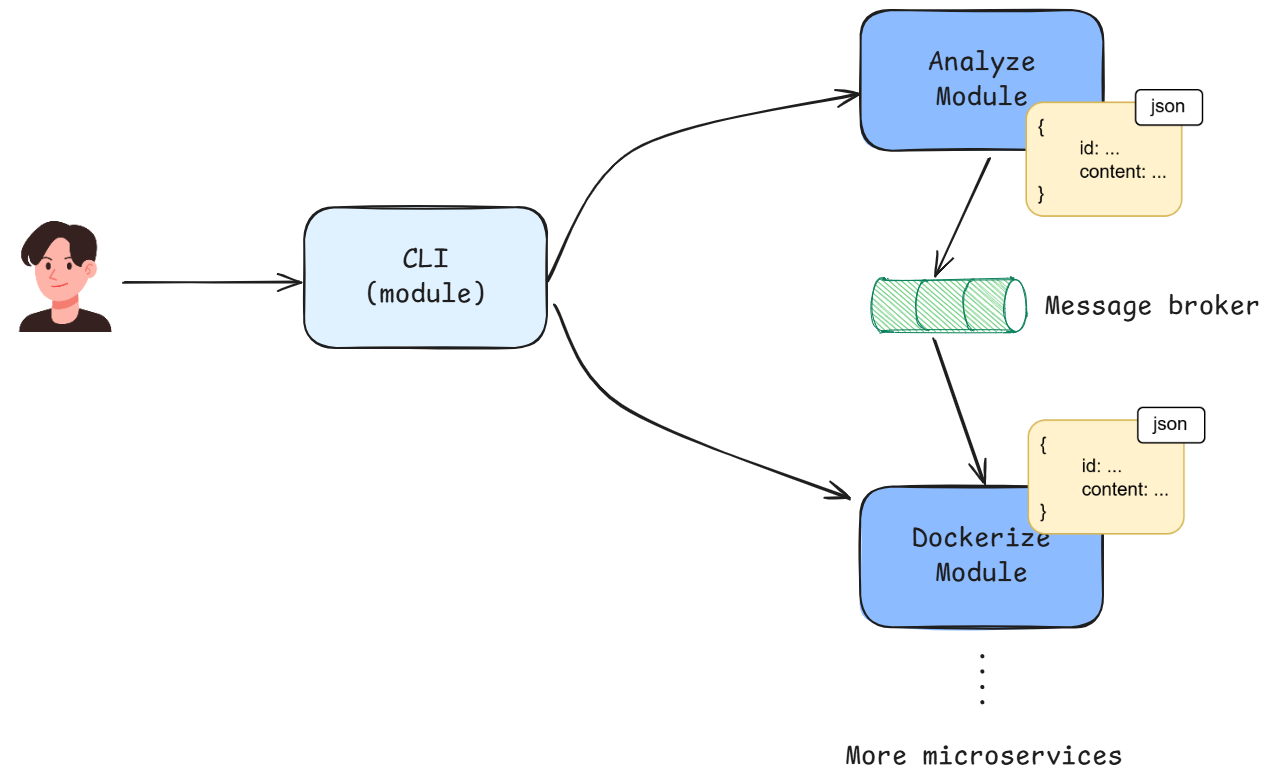
\includegraphics[width=\linewidth]{images/headless-microservice-architecture.png}
    \caption{Headless microservice architecture with microservice-based API}
    \label{fig:headless-microservice-architecture}
\end{figure}

In such a scenario, the CLI and the back-end unit would be detached from each other as in the headless architecture and the back-end unit could be organized into independent and self-deployable services so that more scalability can be achieved in terms of service logic and routing. All the services would communicate with the user through a CLI while between each other they would use Messaging solutions like a Message Broker (e.g., RabbitMQ, Kafka) to exchange data/information.

\subsubsection{Headless Modular architecture}
As an alternative to both Monolithic and Microservice architecture styles, Modular monolith is an approach that combines the advantages of monolith architecture - simplicity and robustness and the benefits of microservices - flexibility and scalability. And as Martin Fowler said in \cite{Fowler-2015}: 

\begin{quote}
    "You shouldn't start a new project with microservices, even if you're sure your application will be big enough to make it worthwhile."
\end{quote}

Modular monolith, as an architecture style, structures the application into independent modules or components that can be worked alone but deployed together. It promotes both modularity and cohesion of the system. Using this style in combination with the Headless architecture style, allows everything to be designed as a module - the CLI and all the back-end units (Analyze and Dockerize) \FigRef{fig:modular-headless-architecture-level-2}. All the modules can communicate through APIs with the CLI and each module can communicate with each other again through API or as in the Headless Microservice architecture communication between modules can be established through messaging.

\begin{figure}[H]
    \centering
    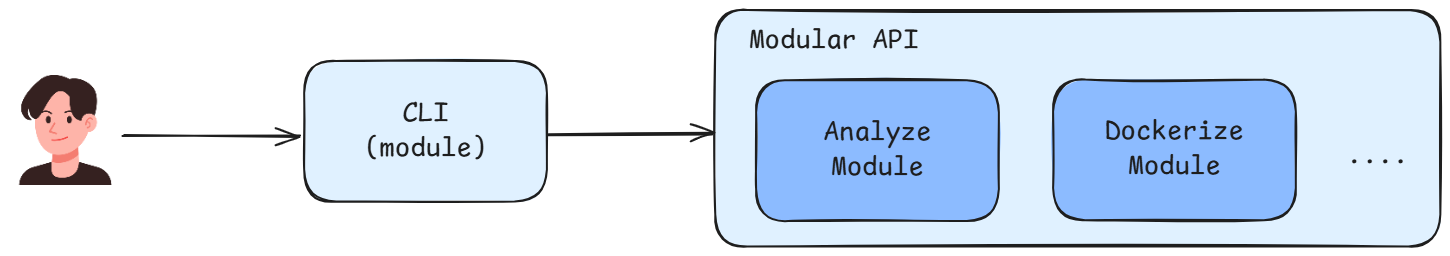
\includegraphics[width=\linewidth]{images/modular-headless-architecture-level-2.png}
    \caption{Modular Headless Architecture with Module-based API}
    \label{fig:modular-headless-architecture-level-2}
\end{figure}

However, this might be seen as a more complex step in the separation of concerns process which is why a rather simpler design was determined to be more appropriate in the current context. It was decided to make use of packages instead of modules for the back-end components - Analyze and Dockerize. This could simplify communication and accomplish more beginner-friendly code organization \FigRef{fig:modular-headless-architecture-level-1}.

\begin{figure}[H]
    \centering
    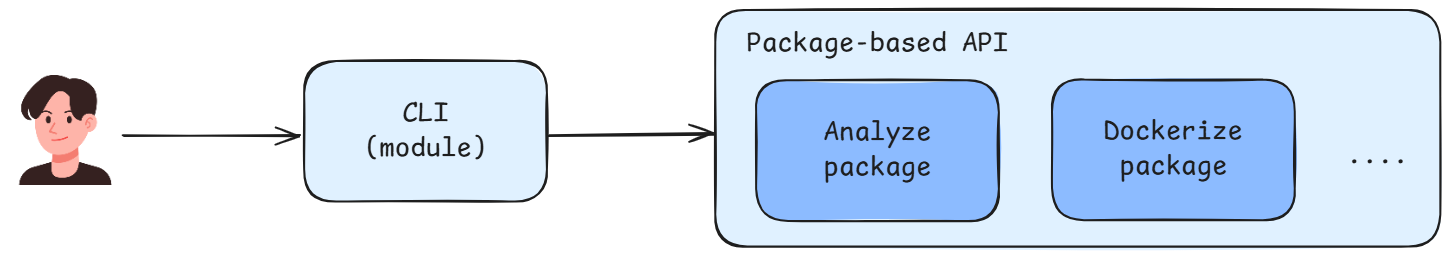
\includegraphics[width=\linewidth]{images/modular-headless-architecture-level-1.png}
    \caption{Modular Headless Architecture with Package-based API}
    \label{fig:modular-headless-architecture-level-1}
\end{figure}

\subsection{System architecture}
Although each of the suggested architectural styles has its advantages and can be employed now or in the future, none of them was selected. It was decided to use a combination of Headless, N-layer monolith, and Modular monolith architecture styles for the system. Inspired by the headless architecture style, the system was divided into two detached parts \FigRef{fig:cli-api-conn}: CLI acting as the front end and API acting as the back end. 

\begin{figure}[H]
    \centering
    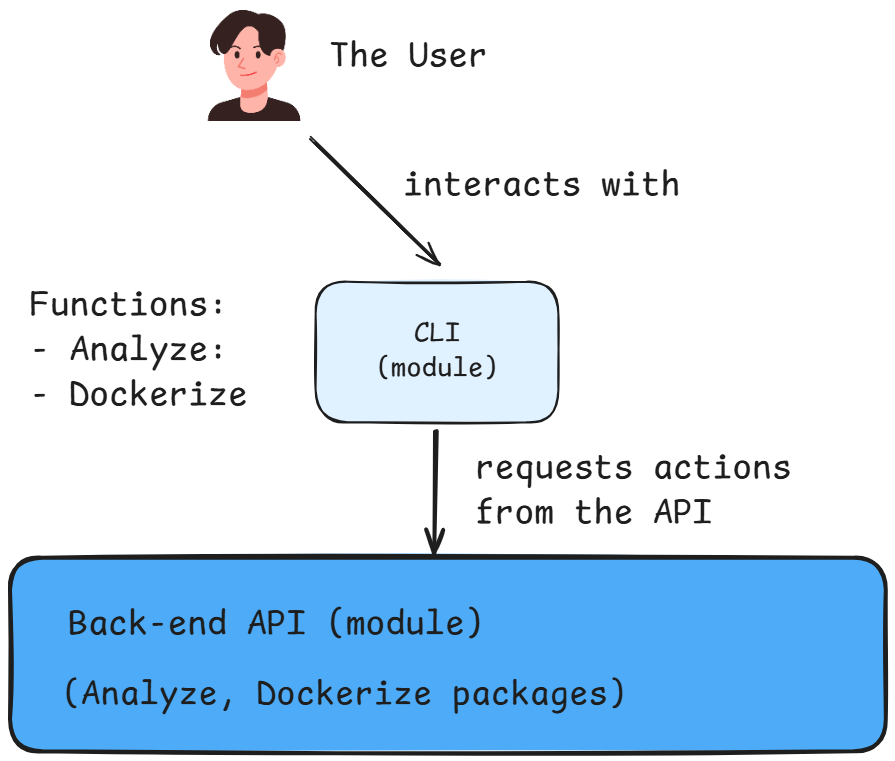
\includegraphics[width=\linewidth]{images/cli-api-connection.png}
    \caption{CLI to API connection}
    \label{fig:cli-api-conn}
\end{figure}

Powered by the Modular architecture style, the two detached system components \FigRef{fig:cli-api-conn}: CLI and API were designed and developed as Golang modules. The API was constructed as a back end that uses layers similarly as in the N-layer architecture \FigRef{fig:back-end-api-layers}: models to store the Data Objects (such as Port, Service) and routes to store the controllers. The service logic was developed in separate files and utilized functions that can be called from the router interface function. As the PoC was developed in Golang, Golang packages were employed to separate each layer but also the different routes in the routes layer. The two main parts of the migration process, "Analyze" and "Dockerize", were introduced as packages, located in the routes layer.

\begin{figure}[H]
    \centering
    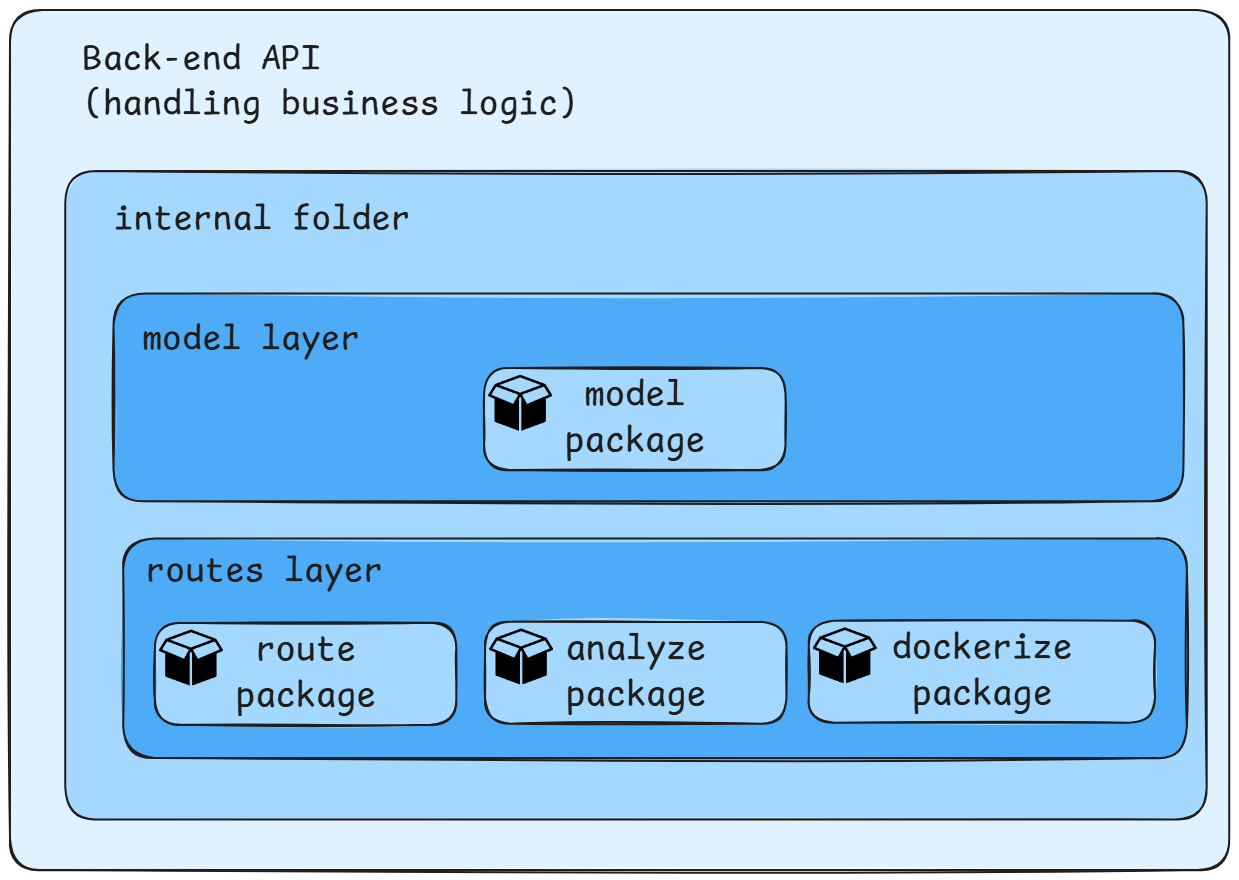
\includegraphics[width=\linewidth]{images/back-end-api-layers.png}
    \caption{Back-end API layers}
    \label{fig:back-end-api-layers}
\end{figure}

\subsubsection{Tech stack}
The system was designed to have two main components, CLI and API, which are detached from each other and can be developed and deployed independently, allowing different technologies to be used for each of them. \\

API technologies such as REST, GraphQL, and gRPC further complement modern architectural trends by facilitating efficient communication between distributed systems \cite{Ali-2024}. While REST remains the most mature and widely adopted API approach, GraphQL and gRPC are increasingly favored for more dynamic, high-performance systems, particularly in real-time applications \cite{Ali-2024}. This shift towards using the right API for the right use case highlights the importance of aligning technical architecture with both current needs and future scalability requirements \cite{Nivedhaa-2024}, \cite{Ali-2024}. Regarding APIs, REST remains the most mature and widely adopted technology, which is why it was chosen for the project and the development of a PoC. There is a long list of modern technologies that can serve the needs to build a professional-made API. \\

The goal of the project from its beginning was to automate the migration of an application from a VM to a container which requires a script-oriented approach to analyze the application profile and run a container based on it. In this research paper, two modern languages (Python and Golang) and one automation tool (Ansible) were considered. \\

As stated in \cite{NanzEtAl-2015} Python as a scripting language enables writing more concise code than procedural languages like Golang and also produces smaller executables, however, Golang is more economical in terms of RAM, less failure-prone, and much faster when there are computing-intensive workloads. The usage of Golang can be efficient if the system is continuously evolving in functionality. \\

Ansible is a well-known agentless tool for automating tasks related to configuration management \cite{Elradi-2023}, it requires only the installation of Python and pip/pipx \cite{Sesto-2022} and can connect to the target machine to perform automation only using SSH \cite{Elradi-2023}. Compared to other similar tools like Puppet, Salt Stack, and Chef, it is much easier to learn and set up Ansible, providing easy-to-read YAML-based syntax \cite{ChoiEtAl-2023} that can improve the developer’s experience. \\

As Ansible is designed to be idempotent, running playbooks multiple times will not change the system's state \cite{ChoiEtAl-2023}, while Bash/Python/Golang-powered scripts will try to install the same package twice for example. While this is very efficient feature in server and system configuration, in the context of the system it does not provide much power as no installation will be performed, but instead, collection of data is the objective. Still, Ansible can be used as a collector of application information because it is agentless (it does not require installing an agent on the target machine to run configuration scripts) \cite{ChoiEtAl-2023}. Ansible coming with built-in modules for the most popular system description units like users, groups, files, and packages \cite{Kumar-2023}, can be effectively used to build a cross-platform compatible collector of application data which can be then analyzed by the core unit of the system and a Docker container be produced as a result. \\

Although Ansible is very flexible for automation, it is not a programming language, nor suitable for building an API. If the business logic is not built in the form of an API, then the system will be packed in a monolithic-alike structure which will produce a heavy binary at the end and will not allow building a more complex software system in the future. On the other hand, Python and Golang are suitable choices even for enterprise-level software and are more than suitable for building APIs that are flexible and scalable. \\

In the end, Golang was chosen as the language to build the PoC, because it is designed to be modular (everything in Golang is a module or package). Golang is quite lightweight and fast and it provides a C++-like interface that is appropriate for migration systems where a lot of interaction with the OS interface is needed. To develop the back end as an API, the popular Golang framework Gin was used to ease the creation of proper routing. To build the CLI the well-known Golang CLI library Cobra was chosen to maintain a professional-like CLI tool. The prototype was written in Golang using Gin for building an API interface for the two main migration units - Analyse and Dockerize. The two parts of the migration process - analyze and dockerize were built as Golang packages to easily communicate with each other. 

\subsection{Software design patterns}
By integrating design patterns in the code base, the solution became more extensible and flexible. The system was modeled with two main migration process units - Analyze and Dockerize to deliver a successful result. There are two methods: file system and process analysis used to create the profile of an application residing in a VM. The Abstract Factory design pattern was implemented with the use of an interface that combines all the methods to build the application profile - application files, ports, and services and then to develop a function that acts as a factory entry point with input of the type of the analysis approach and output of the concrete analysis method implementation \FigRef{fig:abstract-factory-design-pattern}. 

\begin{figure}[H]
    \centering
    \begin{minted}
    [
    xleftmargin=2em,
    numbers=left,
    frame=lines,
    framesep=2mm,
    baselinestretch=1.2,
    fontsize=\footnotesize,
    bgcolor=LightGray,
    breaklines
    ]{golang}
    // Abstract factory design pattern used
    type IAnalyzerFactory interface {
    	collectApplicationFiles(...)
    	collectExposedPorts(...)
    	collectServices(...)
    }
    \end{minted}
    \caption{Asbtract Factory Design pattern}
    \label{fig:abstract-factory-design-pattern}
\end{figure}

The idea of the factory is to create all distinct products by abstracting the actual product creation into concrete factory classes \cite{GammaEtAl-1993} or structures in the context of Golang. The client code interacts with the factory entry point \FigRef{fig:abstract-factory-entry-point} and can choose one variant of the factory product, making all its sub-products/methods to be compatible \cite{GammaEtAl-1993}. In the context of the project, the user can interact with the Factory entry point to choose between file system and process analysis and then all the methods of the chosen "Analyzer" (the chosen analysis approach) will be utilized correctly. For the project, the three methods do not return a product as an output but a string as they return the path to the created file in the case of "collectExposedPorts" and "collectServices" or file system tree in the case of "collectApplicationFiles" \FigRef{fig:abstract-factory-design-pattern}.

\begin{figure}[H]
    \centering
    \begin{minted}
    [
    xleftmargin=2em,
    numbers=left,
    frame=lines,
    framesep=2mm,
    baselinestretch=1.2,
    fontsize=\footnotesize,
    bgcolor=LightGray,
    breaklines
    ]{bash}
    // Abstract Factory Implementation
    func GetAnalyzerFactory(analyzerType string) (IAnalyzerFactory, error) {
    	switch analyzerType {
    	case "fs":
    		return &FsAnalyzerImpl{}, nil
    	case "process":
    		return &ProcessAnalyzerImpl{}, nil
    	case "mixed":
    		return &MixedAnalyzerImpl{}, nil
    	...
    }
    \end{minted}
    \caption{Asbtract Factory Design pattern}
    \label{fig:abstract-factory-entry-point}
\end{figure}

Serving as an extra approach, the mixed analyzer was added to the factory allowing more flexible analysis of the application profile by allowing for each method of the analysis (collection of application files, ports, and services) the user to be able to choose a different strategy - file system or process analyzer. To implement this flexibility of choosing a strategy for analyzing each part of the process, the Strategy design pattern was integrated in the PoC \FigRef{fig:strategy-design-pattern-struct-base}. 

\begin{figure}[H]
    \centering
    \begin{minted}
    [
    xleftmargin=2em,
    numbers=left,
    frame=lines,
    framesep=2mm,
    baselinestretch=1.2,
    fontsize=\footnotesize,
    bgcolor=LightGray,
    breaklines
    ]{golang}
    type MixedAnalyzerImpl struct {
	applicationFileStrategy IAnalyzerFactory
	exposedPortsStrategy    IAnalyzerFactory
	servicesStrategy        IAnalyzerFactory
    }
    // Methods to allow dynamically changing strategies
    func (m *MixedAnalyzerImpl) SetApplicationFileStrategy(strategy IAnalyzerFactory) {
    	m.applicationFileStrategy = strategy
    }
    ...
    \end{minted}
    \caption{Strategy Design pattern struct base}
    \label{fig:strategy-design-pattern-struct-base}
\end{figure}

The concept behind the Strategy pattern is defining a family of algorithms that are interchangeable and can be used as alternatives to each other \cite{GammaEtAl-1993}. In the context of the project, each part of the process could be processed by a different kind of migration strategy, introduced as a mixed migration approach. The PoC was constructed to support two main strategies - file system and process analysis. By using the mixed approach, each strategy can provide its implementation through the template methods \FigRef{fig:strategy-design-pattern-method}. For example, the user can choose to collect the application files using the file system analysis, while for the collection of exposed ports, the process analysis strategy could be utilized. This way the user has more freedom to experiment with which approach the migration is more successful for their scenario and therefore create their own combinations which might turn out to be more successful than the default ones.

\begin{figure}[H]
    \centering
    \begin{minted}
    [
    xleftmargin=2em,
    numbers=left,
    frame=lines,
    framesep=2mm,
    baselinestretch=1.2,
    fontsize=\footnotesize,
    bgcolor=LightGray,
    breaklines
    ]{golang}
    func (m *MixedAnalyzerImpl) collectApplicationFiles(user string, host string, sourceDir string, destinationDir string, privateKeyPath string) (string, error) {
	if m.applicationFileStrategy == nil {
		return "", fmt.Errorf("...")
	}
		return m.
			applicationFileStrategy.
			collectApplicationFiles(
			     user, 
			     host, 
			     sourceDir, 
			     destinationDir, 
			     privateKeyPath,
		      )
    }
    \end{minted}
    \caption{Strategy Design pattern in-method use}
    \label{fig:strategy-design-pattern-method}
\end{figure}

\subsection{User experience}
Although the core part of the system is to make successful VM-to-container migrations, it is compulsory to complement it with a user-friendly design, as otherwise, no one would like to use it. CLI being the primary point of interaction with the user and front end of the system, will be the focus of this results section. \\

CLIs are used primarily by humans and usability should be one of the focus points of their design \cite{Newton-2016}, but usually, they are not designed for humans first, nor do they provide a good level of interaction design \cite{Tiedemann-2023}. The conventions of the UNIX environment such as standard in/out/err, signals, and exit codes ensure different programs work together nicely \cite{Tiedemann-2023}, indicating the system's CLI could become highly flexible if can work with other programs for or related to VM-to-container migrations. \\

Choosing what output the CLI has to provide to the user is important because plain, line-based text can be easily piped between commands, while JSON allows integrations with the web \cite{Tiedemann-2023}, outlining different form of output can serve different purposes. Building the CLI to follow already existing industry patterns, makes the CLI more intuitive \cite{Tiedemann-2023}, \cite{Newton-2016}. As suggested by \cite{Newton-2016} CLI options should be human-readable and supplemented by short aliases like -v for –verbose, but if the user is still unsure how to proceed, an intuitive help command must be provided \cite{Salesforce-2024}. Versioning of the CLI is crucial so that users can easily check if a certain version has a bug report \cite{Salesforce-2024}. A long period without output is not user-friendly according to \cite{Salesforce-2024} and the output has to be designed to be human-readable, offering JSON when needed \cite{PrasadEtAl-2024}. As stated in \cite{Tiedemann-2023}, people should be able to search for CLI documentation through a web interface. To design the CLI to be lightweight, \cite{Salesforce-2024} advises moving as much business logic as possible out of the actual CLI script and utilizing modular code design. \\

A core unit managing the business logic needs to be designed to build a lightweight and user-friendly CLI. The core unit needs to collect the application’s data, analyze it, and create a Dockerfile based on it \FigRef{fig:cli-api-communication}. The CLI could interact with the core unit (back end) to ask for actions (Analyze or Dockerize) and receives outputs based on them.

\begin{figure}[H]
    \centering
    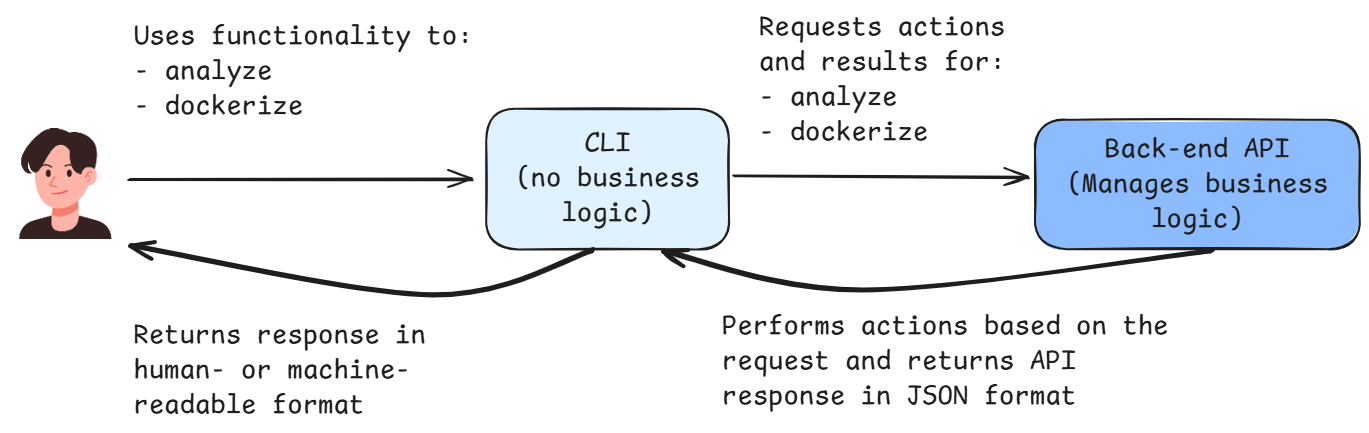
\includegraphics[width=\linewidth]{images/cli-api-communication.png}
    \caption{CLI to API communication}
    \label{fig:cli-api-communication}
\end{figure}

The collection of the application’s data is particularly important to provide a good user experience. Thus, the usage of agentless tools/scripts to collect application data will be a crucial step towards improved user experience and a more lightweight software architecture \FigRef{fig:agentless-collector}.

\begin{figure}[H]
    \centering
    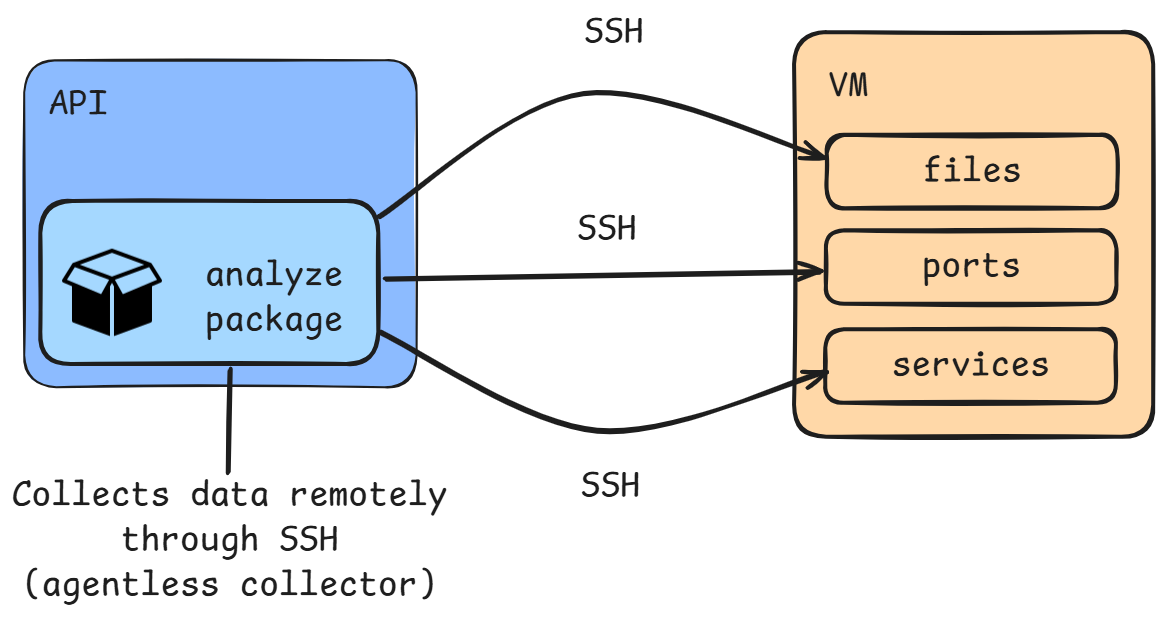
\includegraphics[width=\linewidth]{images/agentless-collector.png}
    \caption{Agentless collector}
    \label{fig:agentless-collector}
\end{figure}

As stated in \cite{Elradi-2023} automation is the way to run tasks without human interventions and the CLI aims to achieve the collection of the application’s data without relying on manual actions from the user such as installing a piece of software on the target VM. To maintain a lightweight and quickly-to-install interface, the CLI was designed as a binary installable that does not contain any service logic and makes requests to the back end through an API interface to gather the results of the analysis and dockerization processes \FigRef{fig:installable-lightweight-cli}. 

\begin{figure}[H]
    \centering
    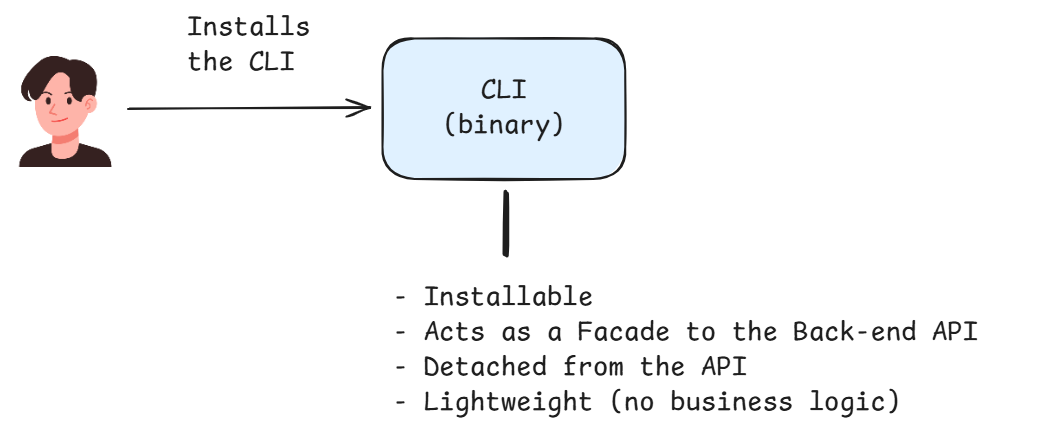
\includegraphics[width=\linewidth]{images/installable-lightweight-cli.png}
    \caption{Installable Lightweight CLI}
    \label{fig:installable-lightweight-cli}
\end{figure}

The CLI was designed with two main commands - analyze and dockerize \FigRef{fig:cli-analyze-command}, \FigRef{fig:cli-dockerize-command}. The first command asks for the following input from the user: type (analysis approach type), user (username of the user to access the VM), host (IP of the VM), privateKeyPath (path to the SSH key to access the VM). The dockerize command asks for the following input: dockerImageName (name of the docker image created from the Dockerfile), dockerContainerName (name of the container created from the docker image). 

\begin{figure}[H]
    \centering
    \begin{minted}
    [
    xleftmargin=2em,
    numbers=left,
    frame=lines,
    framesep=2mm,
    baselinestretch=1.2,
    fontsize=\footnotesize,
    bgcolor=LightGray,
    breaklines
    ]{bash}
    vm2cont analyze \
      --type=fs \
      --user=<username> \
      --host=<IP address> \
      --privateKeyPath=<path to private key>
    \end{minted}
    \caption{CLI Analyze command}
    \label{fig:cli-analyze-command}
\end{figure}

\begin{figure}[H]
    \centering
    \begin{minted}
    [
    xleftmargin=2em,
    numbers=left,
    frame=lines,
    framesep=2mm,
    baselinestretch=1.2,
    fontsize=\footnotesize,
    bgcolor=LightGray,
    breaklines
    ]{bash}
    vm2cont dockerize \     
        --dockerImageName=<docker image name> \
        --dockerContainerName=<docker container name>
    \end{minted}
    \caption{CLI Dockerize command}
    \label{fig:cli-dockerize-command}
\end{figure}

Also, an "output" flag (\FigRef{fig:cli-analyze-command-output})  was added to provide the option for the user to choose between human-readable and machine-readable output. In the current state of the PoC, human-readable output was considered normal text, and machine-readable format was considered JSON.

\begin{figure}[H]
    \centering
    \begin{minted}
    [
    xleftmargin=2em,
    numbers=left,
    frame=lines,
    framesep=2mm,
    baselinestretch=1.2,
    fontsize=\footnotesize,
    bgcolor=LightGray,
    breaklines
    ]{bash}
    vm2cont analyze \
      --type=fs \
      --user=<username> \
      --host=<IP address> \
      --privateKeyPath=<path to private key> \
      --output=<json|text>
    \end{minted}
    \caption{CLI Analyze command with specified output}
    \label{fig:cli-analyze-command-output}
\end{figure}

\subsection{Infrastructure management}
As the system to perform migrations of an application from virtual machine to container was designed to have several components, infrastructure management is an important aspect of the proposed design and prototype. Companies like Sue will most probably need to migrate applications, residing in a private network, which makes it mandatory to have access to this private network to perform any kind of migration. \\

Secure Shell (SSH) being a mechanism for secure connections between Linux hosts \cite{Both-2023}, can be used to access a VM residing in a private network from the back-end API. The back-end API was designed to access the target VM for analysis using only SSH. A system prerequisite is adding a user to the target VM which can access it remotely through SSH connection. Once a user is available, the system will only request the necessary data: username, path to the private SSH key, and host IP of the target VM. If both the VM and the back-end API are located in the same private network they can communicate with each other through their private IP addresses\footnote{IP address - Internet Protocol address, a numerical label that is assigned to a device connected to a computer network that uses the Internet Protocol for communication}. \\

In case the API and the target VM are not located in the same private network, then the VM should expose its public IP so that the system can interact with it to perform analysis. Although this might look straightforward, it opens security issues, because the VM is then exposed to the world through its public IP address. To avoid exposing the target VM through its public IP, a VPN\footnote{VPN - Virtual Private Network, a network architecture for virtually extending a private network across one or multiple other networks which are either untrusted or need to be isolated} connection can be used. A VPN creates an encrypted tunnel between the system and the private network where the target VM is located. The VPN serves as a bridge between the system and the target VM allowing the VM to securely connect to the VM without exposing it to the internet. The VPN connection that could be established is visualized in the diagram on \FigRef{fig:api-vm-connection}. 

\begin{figure}[H]
    \centering
    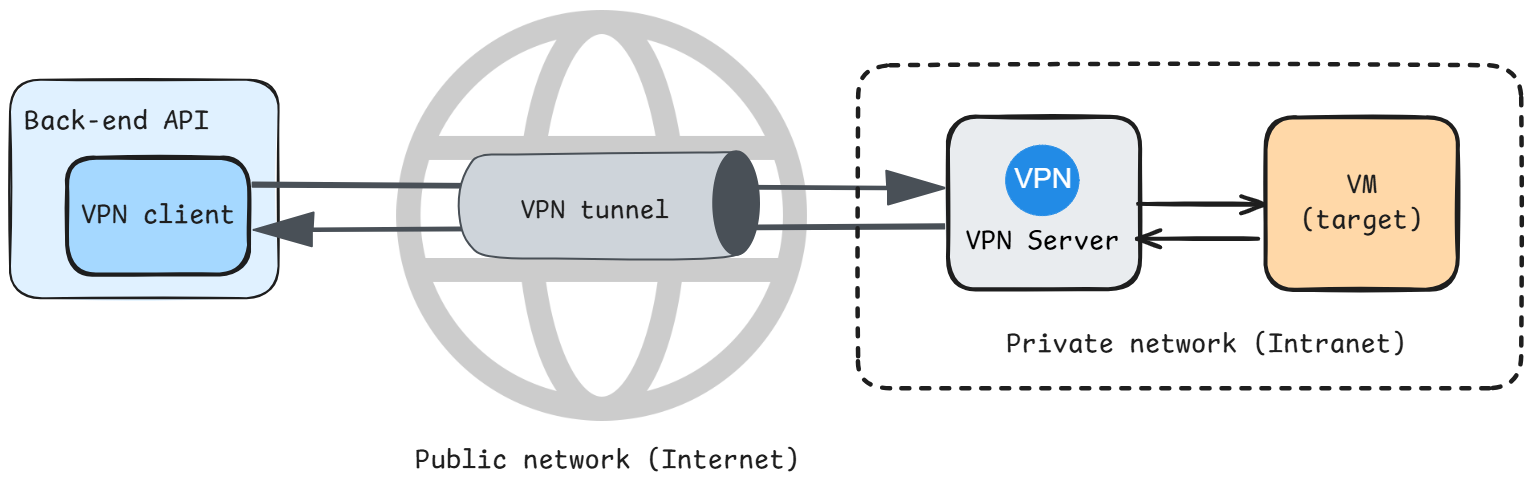
\includegraphics[width=\linewidth]{images/api-vm-connection.png}
    \caption{API to VM Connection}
    \label{fig:api-vm-connection}
\end{figure}

In the private network where all the company's VMs (possible targets for the system) are located, a VPN server should be deployed. Well-known options for a VPN server are WireGuard, and OpenVPN in case self-hosting is preferred. However, managed VPN solutions offered by popular cloud providers can be used to serve the same purposes. Once the VPN server is up and running in the private network, the system can install and configure a VPN client with credentials provided by the VPN server and then request a connection to the target VM through the VPN tunnel. Once the connection is established, the system can freely and securely communicate with the VM.\\

While the system or more specifically the "Analyze package" needs to communicate directly with the VM, the CLI is not going to establish any connections with the target VM, nor perform any commands directly on it. The CLI will only communicate with the back-end API and send API requests to it based on the user inputs. The CLI will act as a "Facade" for the user to not know where and how the back end is deployed and functions as a system component. The concept behind the detached CLI is organized around the idea of providing a lightweight interface to the user and hiding the complexity while focusing on the user experience and on fulfilling the user's requests and needs. \\

Making the CLI available for installation only through a web interface that can be accessed using proper authentication credentials can increase the security of the system and make unwanted access to the system forbidden. Authentication credentials can be received on request from the company's management where the system is integrated.

\subsection{Results summary}
The paper modeled the software architecture and infrastructure design of a system to migrate stateless applications from virtual machines to containers. Through an applied technical experiment, it was concluded that the PoC for the system, implemented based on the software and infrastructure design of the system, produced a successful migration of a Nginx web server from a Ubuntu VM to a Docker container. \\

The full overview of the software architecture design of the system is presented in Appendix \ref{appendix:software-arch-overview-diagram}. In the paper, short code snippets were used to describe different parts of the implementation which supports the findings and results gathered through applied experiments. The full code base of the PoC, demonstrating a software system that can transfer a stateless application such as a web server from an Ubuntu virtual machine to a Docker container, can be found in the GitHub repository of the project (Appendix \ref{appendix:PoC}).

\section{Discussion}
Several months of analysis on the topic of VM-to-container migration showed it is possible to perform a black-box migration of a stateless application from a Linux-flavored VM like Ubuntu to a Docker container in a highly automated way. Moreover, designing an enterprise-level system instead of just a script to conduct the migration of an application from a VM to a container, appeared to be an appropriate approach if the solution aims to be lightweight, user-friendly, extensible, and flexible. The system was designed to ask for minimal input from the user which is why it can be considered as one that performs black-box migration of applications \FigRef{fig:system-overview}.

\begin{figure} [H]
    \centering
    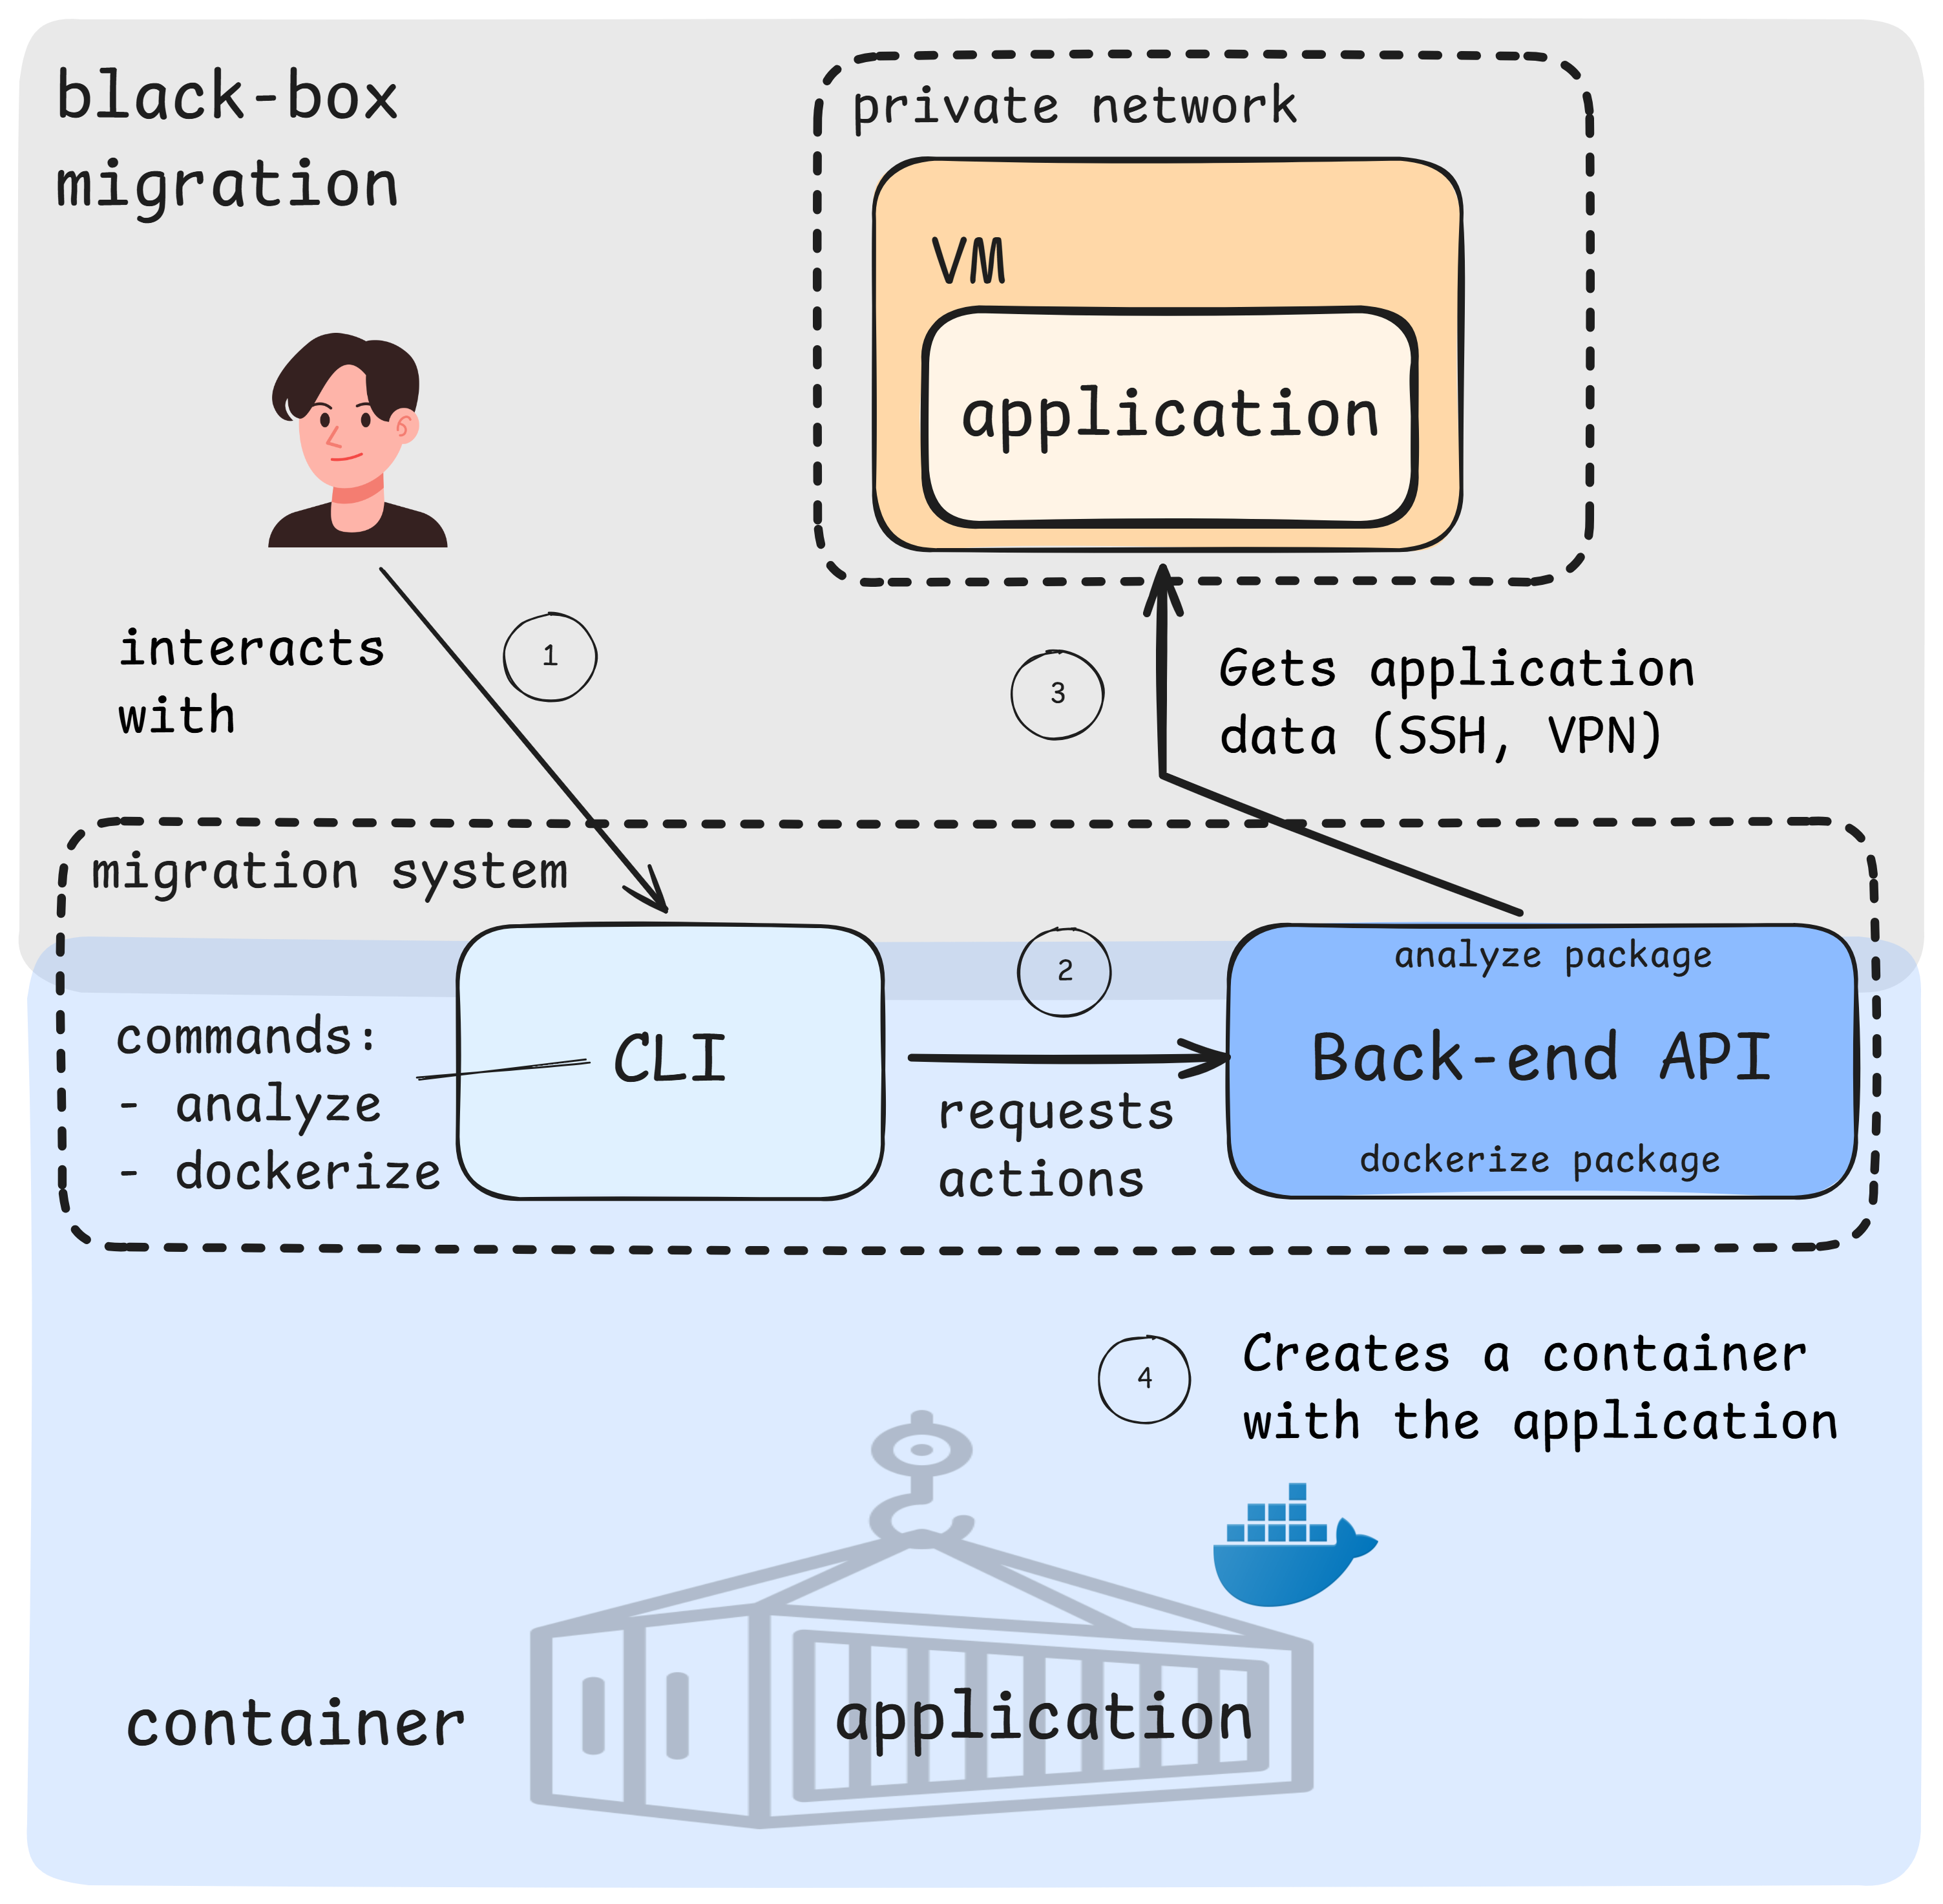
\includegraphics[width=\linewidth]{images/system-overview.png}
    \caption{System overview}
    \label{fig:system-overview}
\end{figure}

In terms of software architecture, the system was designed with two main components: CLI and back-end API where the CLI acts as a lightweight front end that allows the user to interact with the system quickly and easily. The back end handles the business logic and provides outputs/results to the CLI in JSON format so that the CLI can present them to the user. \\

The back end was constructed to perform analysis of an application, located in a VM, then gather the application files, exposed ports, and services to build an application profile. Based on the application profile the back end can generate a Dockerfile, build a Docker image, and run a Docker container with the transferred application. \\

By combining several architecture styles such as Modular Monolith and Headless architecture, the system was organized into two headless modules which allow independent development, deployment, and infrastructure management. The back end was structured into layers and packages, inspired by the N-layer Monolith architecture style and package-based approach of building Golang applications, which results in good readability, separation of concerns, and effortless communication, while also enabling future scalability of the system and its business logic. \\

In terms of application profiling, the PoC of the system focused on the file system analysis, creating a complete example of migrating a Nginx web server from an Ubuntu VM to a Docker container. The other discovered approach for application profiling, process analysis, was not discovered in detail but the system was designed to support it in the future. The system was thought to be highly extensible and to support more than one analysis approach in the future through the use of software design patterns integrated into the code base. In terms of flexibility, the system prototyped an innovative mixed approach to perform analysis by combining the file system and process analysis and allowing the user to choose which approach to use for each part of the process: collection of application files, exposed ports, and services. \\

The CLI was designed based on the modern design best practices in the area of CLI development, following the guidelines of the popular CLI tools, but also keeping the interface intuitive allowing just two options - to analyze the application profile and to dockerize, meaning creating a container for the application based on the application profile. The system was designed to be interpreted by both human users and machine-powered users (i.e., other programs) by integrating both machine- and human-readable formats for the output that the CLI provides to the user. \\

During the study, it was analyzed how the system could be managed in terms of infrastructure in a company environment, and found that the best option is to deploy the back end on a cloud VM or local server while the CLI can be downloaded as a binary/installable from a web interface using authentication credentials, provided by the company's management. To support secure communication without the need to deploy the back end in the same private network as the target VM, the paper suggested deploying a VPN server in the private network where the target VM resides and allowing the back end to communicate with the target VM through a VPN tunnel. \\

While various aspects of designing a complete software system for making a VM-to-container migration were analyzed in the paper, still, the PoC does not dive into detail on how to build a fully functional, secure, and ready-to-be-used system. In terms of functionality, more research and experiments are needed to improve the business logic and be able to perform migrations for more complex applications than web servers, both stateless and stateful ones. Security was not a focus of this work, although it was partially covered in the Infrastructure management section, which is why this opens a space for future research-oriented experiments on how the system can be protected from malware access and theft of sensitive data. This paper focuses more on designing the full overview of a system that can do an automated migration and does not examine the performance of both analysis approaches, which can be another topic of future research. \\

While these limitations do not affect the current results of designing a software system to migrate a stateless application from a VM to a container, future work is needed to continue what was discovered and further enhance the business logic to perform more complex migrations.

\section{Conclusion}
The paper designed and prototyped an enterprise-level software system that performs automated VM-to-container migrations to help companies move their or their clients' legacy applications from old-fashioned virtual machine environments to more lightweight, portable, and operationally efficient container environments. \\

A migration process consisting of two parts Analyze and Dockerize was modeled where the first one is responsible for analyzing the target VM and creating an application profile while the second one has to generate a Dockerfile out of the profile, build a Docker image and run a Docker container to verify a successful migration was performed. Using file system analysis, the PoC developed during the study, performed a successful migration of a Nginx web server from Ubuntu VM to a Docker container. Additionally, the system was designed to support the other type of analysis approach - process analysis. \\

A topic of future research could be the migration of more complex stateless and stateful applications as the current solution is limited to making migrations of web servers. Another limitation of the current solution is the security of the system which is not covered as a separate sub-topic, although it was considered while modeling the infrastructure management plan for the system. \\

These limitations could be a useful next step but do not affect the current results which showed designing a system to perform migrations requires many aspects of the problem to be worked but it brings many benefits such as better user experience, more extensible, flexible, and easier-to-maintain business logic that allows more and combination of different migration approaches to be employed.

\section{Acknowledgments}
The paper was written under the academic guidance of Casper Schellekens, a teacher at the Master of Applied IT at Fontys University. Through the project, feedback and expert evaluation sessions on the topic of software architecture were also organized with colleagues of Casper, the teachers Simona Orzan, and Nico Kuijpers. These sessions helped to find the right direction and complete the paper. Besides Fontys, Sue acted as a sponsor of the project, and the Product owner of the research project, Nathan Keyaerts from Sue, provided continuous technical and academic feedback used to dive deep into the topic and to fine-tune the paper's findings and results in the end.

\printbibliography

\onecolumn
\begin{appendices}
\section{Software architecture overview diagram}
\label{appendix:software-arch-overview-diagram}
\begin{figure}[hbt]
    \centering
    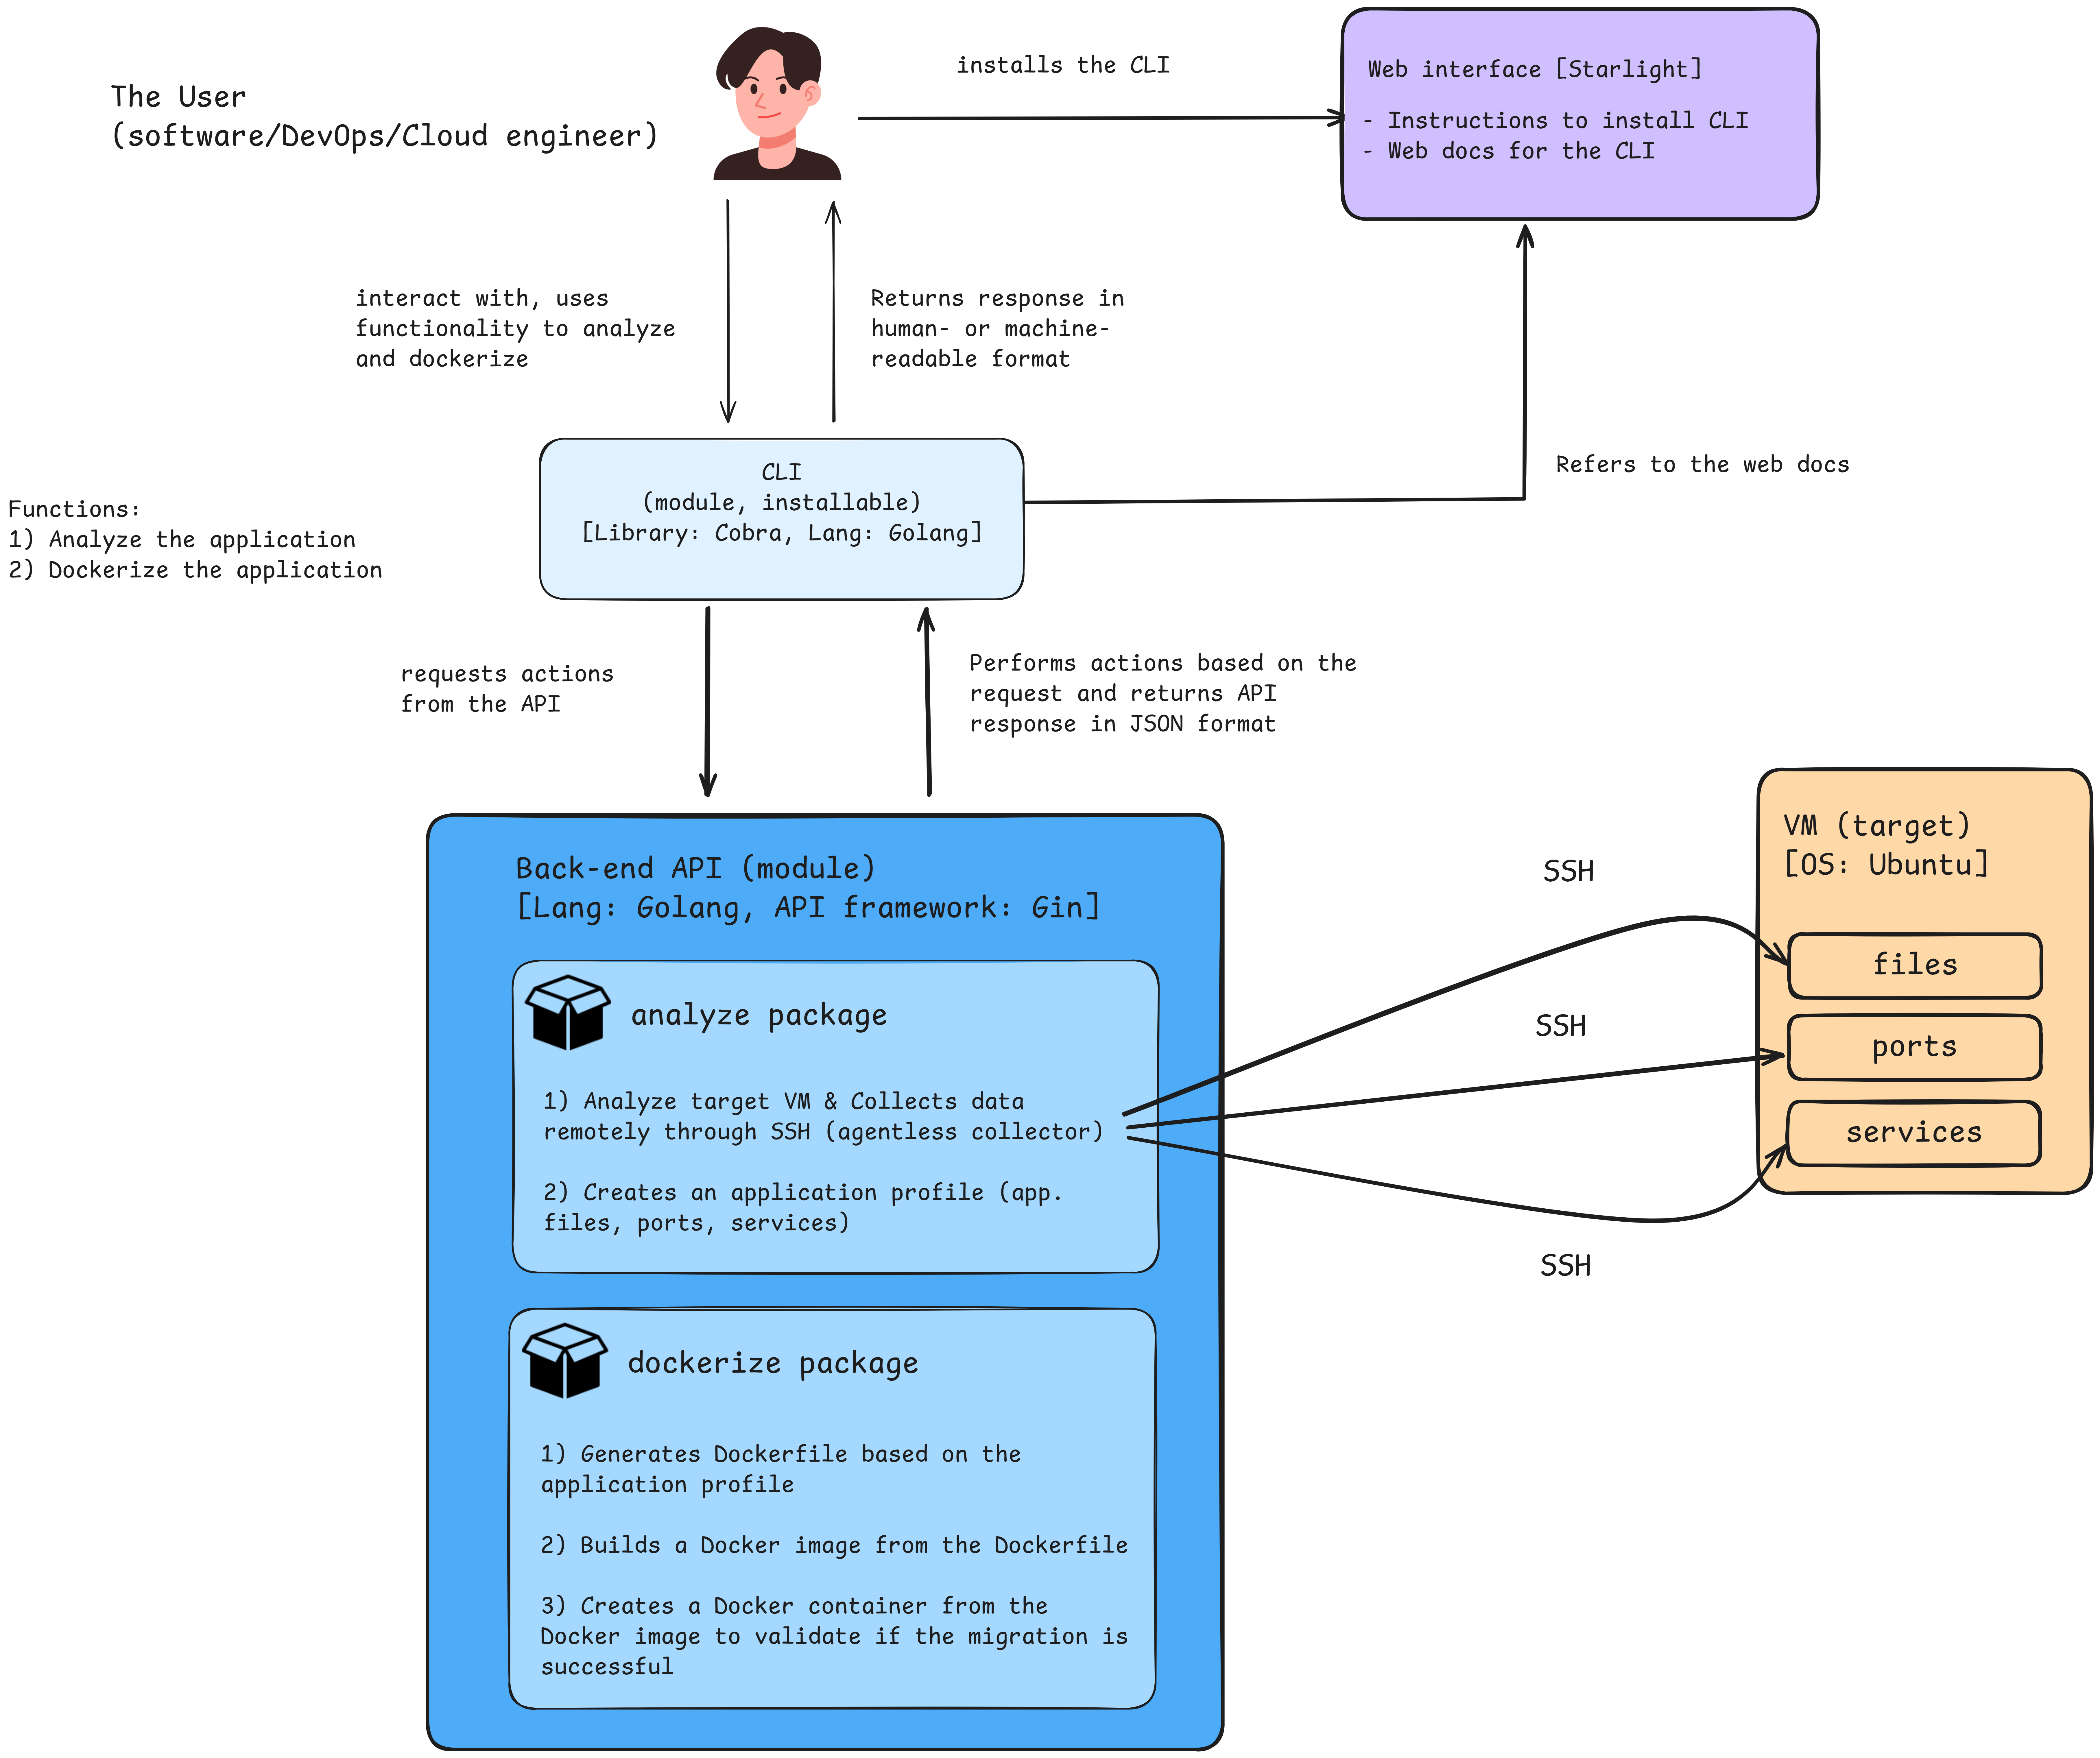
\includegraphics[width=\linewidth]{images/software-architecture-overview.png}
    \caption{Software architecture overview diagram}
\end{figure}

\section{Software system PoC}
\label{appendix:PoC}
The code for PoC for a Software system to migrate stateless applications from a VM to a container can be found in: \href{https://github.com/toni123321/vm-to-container-migrator}{https://github.com/toni123321/vm-to-container-migrator}
\end{appendices}

\end{document}